\documentclass[a4paper,11pt]{article}
\usepackage{amsmath,latexsym}
\usepackage{geometry}
\usepackage{graphicx}
\linespread{1.2}
\geometry{left=2.5cm,right=2.5cm,top=2.5cm,bottom=2.5cm}
\begin{document}
\title{\Large{$SFM01-VaR-blockmaxima-backtesting$}}
\date{July 13th, 2016}
\maketitle
\begin{flushleft}

Project members:\\

Liang chen 15620151152901\\Du yao 15620151152897\\Feng xiaowei 15520151152644\\Zi xuefei 15620151152919\\

Data source: $http://en.boerse-frankfurt.de$\\

Data range: all the trading days from $2002-01-01$ to $2016-06-30$, daily data.\\

Data files: $Bayer-close-0216.txt$,$Bmw-close-0216.txt$,$Siemens-close-0216.txt$.\\

Steps of procedure:\\

1.construct a portfolio: $V=Bayer+Bmw+Siemens$.\\

2.Calculate the $VaR$ of the portfolio by using Block Maxima Model.\\

  (1)Decompose negative returns $\{X_t\}_{t=1}^T$ into $k$ non-overlapping sets.\\
  
  (2)Define $\{Z_j\}_{j=1}^k$ where $Z_j=max\{X_{(j-1)n+1},...,X_{jn}\}$.\\
  
  (3)For $\{Z_j\}_{j=1}^k$, fit generalized extreme value distribution $G_{\gamma}(\frac{x-\mu}{\sigma})$.\\
  
  (4)$VaR$ at $\alpha$: $VaR(\alpha)=\mu+\frac{\sigma}{\gamma}[(-log(1-\alpha^n))^{-\gamma}-1]$.\\
  T denotes the number of observations.\\
  
3.Backtesting with Moving Window Method.\\

  (1)Daily P\&L of the portfolio from $2002-01-01$ to $2016-06-30$.\\
  
  (2)Static windows of size $h=250$ scrolling in time $t$ for $VaR$ estimation $\{X_t\}_{t=s-h+1}^{s}$ for $s=h,...,T$.\\
  
  (3)Moving window results: Estimates of the parameters of $G_{\gamma}(\frac{x-\mu}{\sigma})$ by MLE, that is, $\{\hat{\mu}_t\}_{t=h}^T$, $\{\hat{\sigma}_t\}_{t=h}^T$, $\{\hat{\gamma}_t\}_{t=h}^T$, and $\{\widehat{VaR}_{1-\alpha}^t\}_{t=h}^T$.\\
  
  (4)Take the opposites of $\{\widehat{VaR}_{1-\alpha}^t\}_{t=h}^T$ and find the outliers.\\
  
4.Calculate exceedances ratio\\
$$\hat{\alpha}=\frac{1}{T-h}\sum_{t=h+1}^{T}I\{X_t<-\widehat{VaR}_{1-\alpha}^{t}\}$$\\

5.Realizations by R and Matlab.\\

  (1)Value-at-Risk estimation at $\alpha = 0.05$ level for portfolio, with size of moving window $h=250$ and size of block $n = 16$.\\

  (2)Backtesting result with R: $\hat{\alpha}= 0.0495$.\\

  (3)Backtesting result with Matlab: $\hat{\alpha}= 0.0501$.\\

  (4)The difference is caused by the different estimation procedure of GEV in the two softwares.\\

\begin{figure}[htpb!]
      \centering
      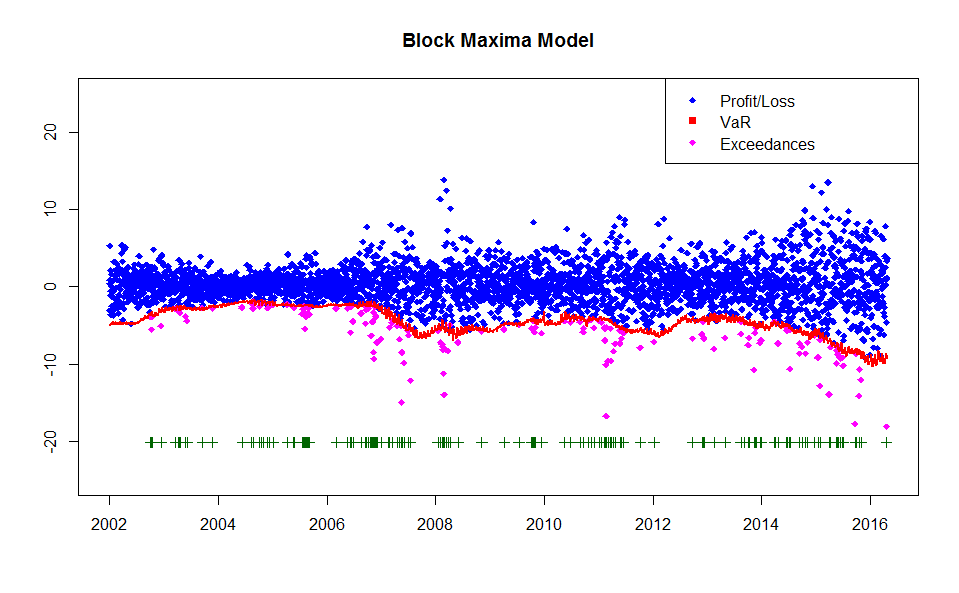
\includegraphics[width=12cm,height=9cm]{VaR_BBM_backtesting_R.png}
      \caption{$VaR-BBM-backtesting-R$}
\end{figure}
\begin{figure}[htpb!]
        \centering
        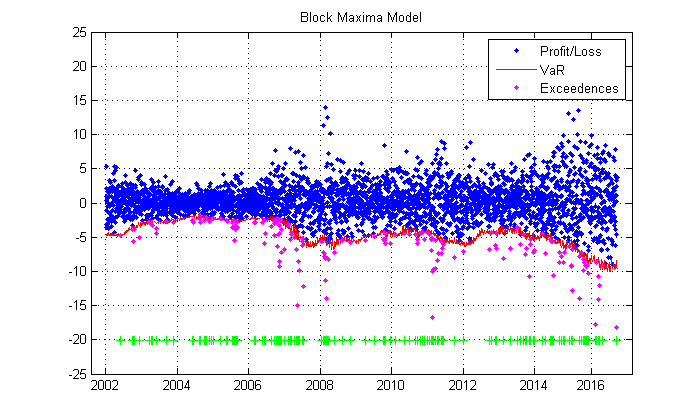
\includegraphics[width=12cm,height=9cm]{VaR_BBM_backtesting_Matlab.png}
        \caption{$VaR-BBM-backtesting-Matlab$}
\end{figure}
\end{flushleft}
\end{document}



